\documentclass[12pt]{exam}
% Package imports
\usepackage{multicol}
\usepackage{amsmath, amsthm, amssymb, fullpage}
\usepackage[a4paper,left=1.5cm,top=1.5cm,right=1.5cm,bottom=2cm]{geometry}
\usepackage{amsfonts}
\usepackage[utf8]{inputenc}
\usepackage{breqn}
\usepackage[hidelinks]{hyperref}
\usepackage{hyperref}
\usepackage{afterpage}
\usepackage{longtable}
\usepackage{indentfirst} 
\usepackage[table,xcdraw]{xcolor}
\usepackage{caption}
\usepackage{subcaption}
\usepackage{graphicx}
\usepackage{titlesec}
\usepackage{biblatex}
\usepackage{graphicx}
\usepackage{float}
\usepackage{makecell}
\usepackage{multicol}
\usepackage{array, multirow}
\usepackage{tikz}
\usepackage{booktabs}
\usepackage{array}
\usepackage{enumitem}
\usepackage{pgfplots}
\renewcommand{\questionlabel}{\textbf{\thequestion.}} 
\usepackage{booktabs}
\usepackage{pgfplots}
\pgfplotsset{compat=1.18}
\setlength{\columnsep}{1.5cm}
\setlength{\tabcolsep}{10pt}
\usepackage{array}
\usepackage{background}
\backgroundsetup{
  scale=1.5,
  position=current page.center,
  opacity=0.1,
  angle=0,
  contents={\includegraphics{images/watermark.png}}
}
\usepackage{xcolor}
\pagestyle{headandfoot}
\definecolor{RAL3003}{RGB}{155, 17, 30}
\firstpagefooter{\vspace{-3mm}\textbf{\textcolor{RAL3003}{\href{https://t.me/satashkent}{@satashkent}}}}{}{\vspace{-3mm}\textbf{\textcolor{RAL3003}{\thepage}}}  
\runningfooter{\vspace{-3mm}\textbf{\textcolor{RAL3003}{\href{https://t.me/satashkent}{@satashkent}}}}{}{\vspace{-3mm}\textbf{\textcolor{RAL3003}{\thepage}}}  
\begin{document}
\title{Linear Functions}
\begin{enumerate}
    % Page 1
    \item The function $m$ is defined by $m(x) = 30x + 120$. What is the slope of the graph of $y = m(x)$ in the $xy$-plane?
    % Page 2
    \item Lucia and John will work together to make 60 paper flowers for a school party. The line shown represents the possible combinations of time, in hours, spent by Lucia and John to fulfill this task. According to the graph, on average, how many paper flowers will Lucia make per hour?
    \begin{enumerate}[label=\Alph*)]
        \item 4
        \item 5
        \item 12
        \item 15
    \end{enumerate}
    % Page 3
    \item The table shows a linear relationship between $x$ and $y$:
    \begin{center}
        \begin{tabular}{|c|c|}
            \hline
            $x$ & $y$ \\
            \hline
            0 & $n$ \\
            4 & $n + 19$ \\
            8 & $n + 38$ \\
            \hline
        \end{tabular}
    \end{center}
    What is the slope of the line?
    % Page 4
    \item For the linear function $f$, the graph of $y = f(x)$ passes through (0,2) and (3,3). What is the slope?
    % Page 7
    \item In the $xy$-plane, the graph of the linear function $f$ contains (5,7) and (3,11). Which equation defines $f$?
    \begin{enumerate}[label=\Alph*)]
        \item $f(x) = \frac{1}{2}x + \frac{9}{2}$
        \item $f(x) = -\frac{1}{2}x + \frac{19}{2}$
        \item $f(x) = 2x - 3$
        \item $f(x) = -2x + 17$
    \end{enumerate}
    % Page 8
    \item For the linear function $f$, the graph of $y = f(x)$ passes through (0,5) and (7,7). What is the slope?
    % Page 9
    \item Which equation is the most appropriate linear model for the data shown?
    \begin{enumerate}[label=\Alph*)]
        \item $y = -2x$
        \item $y = -x$
        \item $y = x$
        \item $y = 2x$
    \end{enumerate}
    % Page 10
    \item The function $g(m) = -0.05m + 14.1$ models gallons of gasoline remaining after driving $m$ miles. About how many gallons are used per mile?
    \begin{enumerate}[label=\Alph*)]
        \item 0.05
        \item 14.1
        \item 20
        \item 282.0
    \end{enumerate}
    % Page 11
    \item The function $f(m) = 30 - 6m$ gives the money in an account after renting $m$ movies. What represents the amount withdrawn per rental?
    \begin{enumerate}[label=\Alph*)]
        \item $6m$
        \item 6
        \item 30
        \item $30 - 6m$
    \end{enumerate}
    % Page 12
    \item A linear function $f$ gives profit for selling $x$ items: $320 at 6 items, $640 at 10 items. Which equation defines $f$?
    \begin{enumerate}[label=\Alph*)]
        \item $f(x) = 180x - 640$
        \item $f(x) = 64x$
        \item $f(x) = 80x - 10$
        \item $f(x) = 80x - 160$
    \end{enumerate}
    % Page 13
    \item The table shows Adriana's travel time:
    \begin{center}
        \begin{tabular}{|c|c|}
            \hline
            Distance (miles) & Time (minutes) \\
            \hline
            0.06 & 3 \\
            0.28 & 14 \\
            0.34 & 17 \\
            \hline
        \end{tabular}
    \end{center}
    Which equation represents the linear relationship?
    \begin{enumerate}[label=\Alph*)]
        \item $t = \frac{1}{50}d$
        \item $t = \frac{1}{2}d$
        \item $t = 2d$
        \item $t = 50d$
    \end{enumerate}
    % Page 14
    \item The function $w(t) = 600 - 8t$ models water volume draining from a container. What is the volume draining per second (in mL)?
    % Page 15
    \item The function $g(m) = -0.04m + 16.6$ models gasoline remaining after driving $m$ miles. About how many gallons are used per mile?
    \begin{enumerate}[label=\Alph*)]
        \item 0.04
        \item 16.6
        \item 25
        \item 415.0
    \end{enumerate}
    % Page 16
    \item One equation $y = \frac{5}{7}x + 9$ has infinitely many solutions. What is the slope of the second equation?
    \begin{enumerate}[label=\Alph*)]
        \item $-\frac{7}{5}$
        \item $-\frac{5}{7}$
        \item $\frac{5}{7}$
        \item $\frac{7}{5}$
    \end{enumerate}
    % Page 17
    \item The function $T(x) = 62 - 8x$ estimates temperature $x$ hours after 10 a.m. What is the estimated temperature decrease per hour?
    \begin{enumerate}[label=\Alph*)]
        \item 4
        \item 8
        \item 54
        \item 62
    \end{enumerate}
    % Page 18
    \item For linear functions $p$ and $t$: $p(c) = -6$, $p(3) = 26$, slope of $p$ is 8; $t(c) = -7$, $t(4) = 38$. What is the slope of $t$?
    \begin{enumerate}[label=\Alph*)]
        \item -1
        \item 2
        \item 8
        \item 9
    \end{enumerate}
    % Page 19
    \item What is the slope of $y = \frac{1}{2}(11x + 16) + 4x$?
    \begin{enumerate}[label=\Alph*)]
        \item $\frac{11}{2}$
        \item $\frac{19}{2}$
        \item 11
        \item 15
    \end{enumerate}
    % Page 20
    \item Line $r$ has slope 2 and passes through (0,12). Which equation defines $r$?
    \begin{enumerate}[label=\Alph*)]
        \item $y = -12x + 2$
        \item $y = 12x + 2$
        \item $y = 2x - 12$
        \item $y = 2x + 12$
    \end{enumerate}
    % Page 21
    \item The table shows roof area vs. water drained:
    \begin{center}
        \begin{tabular}{|c|c|}
            \hline
            Area (sq ft) & Water (gallons) \\
            \hline
            2,520 & 4,536 \\
            3,780 & 6,804 \\
            5,040 & 9,072 \\
            \hline
        \end{tabular}
    \end{center}
    Which equation could define $f$?
    \begin{enumerate}[label=\Alph*)]
        \item $f(x) = 0.6x$
        \item $f(x) = 1.8x$
        \item $f(x) = 2,268.0x$
        \item $f(x) = \frac{x}{6}$
    \end{enumerate}
    % Page 22
    \item Line $t$ has slope $\frac{1}{3}$ and passes through (15,-6). Which equation defines line $t$?
    \begin{enumerate}[label=\Alph*)]
        \item $y = -11x + \frac{1}{3}$
        \item $y = \frac{x}{3} - 11$
        \item $y = \frac{x}{3} - 6$
        \item $y = 15x - 6$
    \end{enumerate}
    % Page 23
    \item The function $f(m) = 21 - 3m$ gives money in an account after renting $m$ movies. What represents the amount withdrawn per rental?
    \begin{enumerate}[label=\Alph*)]
        \item $3m$
        \item 3
        \item 21
        \item $21 - 3m$
    \end{enumerate}
    % Page 24
    \item What is the slope of $y = \frac{1}{2}(15x + 12) + 3x$ in the $xy$-plane?
    % Page 25
    \item A line has $x$-intercept (-2,0) and $y$-intercept (0,-4). What is the slope?
    \begin{enumerate}[label=\Alph*)]
        \item $-2$
        \item $-\frac{1}{2}$
        \item $\frac{1}{2}$
        \item $2$
    \end{enumerate}
    % Page 26
    \item What is the slope of $y = -11x - \frac{2}{5}(18 - 6x)$?
    % Page 27
    \item A line with slope $\frac{1}{3}$ passes through (-1,1) and (5,n). What is $n$?
    \begin{enumerate}[label=\Alph*)]
        \item 9
        \item 4
        \item 3
        \item $\frac{7}{3}$
    \end{enumerate}
    % Page 28
    \item If line $l$ is $y = mx + b$, which must be true about $mb$?
    \begin{enumerate}[label=\Alph*)]
        \item $mb > 0$
        \item $mb < 0$
        \item $mb = 0$
        \item $mb = 1$
    \end{enumerate}
    % Page 29
    \item What is the slope of the graph of $f$ shown?
    \begin{enumerate}[label=\Alph*)]
        \item $-2$
        \item $-\frac{1}{2}$
        \item $\frac{1}{4}$
        \item $\frac{1}{2}$
    \end{enumerate}
    % Page 30
    \item Linear function $f(x) = ax + b$ has slope 6 and passes through (-5,-14). What is $b$?
    % Page 31
    \item The table shows a linear relationship:
    \begin{center}
        \begin{tabular}{|c|c|}
            \hline
            $x$ & $y$ \\
            \hline
            -6 & $-114 - p$ \\
            -2 & $-57 - p$ \\
            2 & $-p$ \\
            \hline
        \end{tabular}
    \end{center}
    What is the slope?
    \begin{enumerate}[label=\Alph*)]
        \item $-\frac{57}{4}$
        \item $\frac{57}{4}$
        \item $\frac{p - 57}{-4}$
        \item $\frac{2p + 57}{4}$
    \end{enumerate}
    % Page 32
    \item The function $f(x) = 24 + 6x$ models tray weight with $x$ glasses. How many ounces per glass?
    \begin{enumerate}[label=\Alph*)]
        \item 4
        \item 6
        \item 12
        \item 24
    \end{enumerate}
    % Page 33
    \item $w(x) = 100 - 3x$ gives water level in an aquarium. Interpret the slope.
    \begin{enumerate}[label=\Alph*)]
        \item Water decreases by 3 feet/day
        \item Water increases by 3 feet/day
        \item Water decreases by 100 feet/day
        \item Water increases by 100 feet/day
    \end{enumerate}
    % Page 34
    \item In $s = 10 - 2h$, what is the meaning of 2?
    \begin{enumerate}[label=\Alph*)]
        \item Add 2 tsp sugar per tsp honey
        \item Subtract 2 tsp sugar per tsp honey
        \item Add 1 tsp sugar per 2 tsp honey
        \item Subtract 1 tsp sugar per 2 tsp honey
    \end{enumerate}
    % Page 35
    \item In $h = 100 - 4t$, interpret 4.
    \begin{enumerate}[label=\Alph*)]
        \item Increase of 1°C makes milk sour 4 hours faster
        \item Increase of 1°C makes 4 gallons sour 1 hour faster
        \item Increase of 4°C makes milk sour 1 hour faster
        \item Increase of 4°C makes milk sour 4 hours faster
    \end{enumerate}
    % Page 36
    \item In $p = 2,000s + 15,000$, interpret 2,000.
    \begin{enumerate}[label=\Alph*)]
        \item Avg students per school
        \item Avg schools per town
        \item Population increase per additional school
        \item Population without schools
    \end{enumerate}
    % Page 37
    \item In $A = 30 + 40h$, what does 40 represent?
    \begin{enumerate}[label=\Alph*)]
        \item Hours of labor
        \item Flat fee
        \item Charge per hour
        \item Total charge for $h$ hours
    \end{enumerate}
    % Page 38
    \item Values of linear function $f$:
    \begin{center}
        \begin{tabular}{|c|c|}
            \hline
            $x$ & $f(x)$ \\
            \hline
            0 & -2 \\
            2 & 4 \\
            6 & 16 \\
            \hline
        \end{tabular}
    \end{center}
    What is $f(3)$?
    \begin{enumerate}[label=\Alph*)]
        \item 6
        \item 7
        \item 8
        \item 9
    \end{enumerate}
    % Page 39
    \item In $f(p) = 7,000 - 30p$, interpret 30.
    \begin{enumerate}[label=\Alph*)]
        \item $1 price increase \to 30$ fewer players/week
        \item $1 price increase \to 30$ more players/week
        \item $30 price increase \to 1$ fewer player/week
        \item $30 price increase \to 1$ more player/week
    \end{enumerate}
    % Page 40
    \item What is the slope of $3x - 5y = 18$?
    % Page 41
    \item Which equation has a slope of 3?
    \begin{enumerate}[label=\Alph*)]
        \item $y = \frac{1}{3}x$
        \item $y = x - 3$
        \item $y = 3x + 2$
        \item $y = 6x + 3$
    \end{enumerate}
    % Page 42
    \item In $w = 1.2c + 13$, interpret 1.2.
    \begin{enumerate}[label=\Alph*)]
        \item Weight of 1 club
        \item Weight of 13 clubs
        \item Weight of bag (no clubs)
        \item Weight of bag with 13 clubs
    \end{enumerate}
    % Page 43
    \item What is the slope through (0,0) and (3,4)?
    \begin{enumerate}[label=\Alph*)]
        \item $\frac{3}{4}$
        \item $\frac{4}{3}$
        \item 3
        \item 4
    \end{enumerate}
    % Page 44
    \item Canoe rental costs:
    \begin{center}
        \begin{tabular}{|c|c|}
            \hline
            Hours ($x$) & Cost ($y$) \\
            \hline
            1 & 9 \\
            2 & 11 \\
            6 & 19 \\
            8 & 23 \\
            \hline
        \end{tabular}
    \end{center}
    What is the slope?
    \begin{enumerate}[label=\Alph*)]
        \item $\frac{1}{2}$
        \item 1
        \item 2
        \item $2\frac{1}{2}$
    \end{enumerate}
    % Page 45
    \item The line graphed in the xy-plane below models the
total cost, in dollars, for a cab ride, y,, in a certain
city during nonpeak hours based on the number of
miles traveled, x.
    \begin{center}
        \centering
        \includegraphics[width=0.5\linewidth]{Screenshot 2025-06-24 at 19.17.15.png}
    \end{center}
    \begin{enumerate}[label=\Alph*)]
        \item $2.00
        \item $2.60
        \item $3.00
        \item $5.00
    \end{enumerate}
    % Page 46
    \item Values for $h$:
    \begin{center}
        \begin{tabular}{|c|c|}
            \hline
            $x$ & $h(x)$ \\
            \hline
            -7 & -11 \\
            2 & 7 \\
            4 & 11 \\
            \hline
        \end{tabular}
    \end{center}
    What is $h(8)$?
    \begin{enumerate}[label=\Alph*)]
        \item 15
        \item 19
        \item 21
        \item 22
    \end{enumerate}
    % Page 47
    \item Which form displays the slope as a constant or coefficient?
    \begin{enumerate}[label=\Alph*)]
        \item $25 + 11x - y = -4x + 4y$
        \item $-6x + 2y = 10$
        \item $y = 3(x - 2) + 11$
        \item $10x - 4y = -20 - 2x$
    \end{enumerate}
    % Page 48
    \item In $21h + 10c = 900$, interpret 21.
    \begin{enumerate}[label=\Alph*)]
        \item Earnings per hour at regular job
        \item Earnings per hour at second job
        \item Hours at regular job
        \item Hours at second job
    \end{enumerate}
    % Page 49
    \item Line $\ell$ passes through (0,r) and (s,0). What is its slope?
    \begin{enumerate}[label=\Alph*)]
        \item $-\frac{r}{s}$
        \item $\frac{r}{s}$
        \item $-\frac{s}{r}$
        \item $\frac{s}{r}$
    \end{enumerate}
    % Page 50
    \item Line $y = kx + 4$ contains (c,d). What is slope in terms of c and d?
    \begin{enumerate}[label=\Alph*)]
        \item $\frac{d - 4}{c}$
        \item $\frac{c - 4}{d}$
        \item $\frac{4 - d}{c}$
        \item $\frac{4 - c}{d}$
    \end{enumerate}
    % Page 51
    \item Line $k$ has slope $-\frac{2p}{5}$ and $y$-intercept (0,p). What is the $x$-coordinate of the $x$-intercept?
    % Page 52
    \item For $g(x) = \frac{4}{5}x - 32$, what is the $x$-intercept?
    % Page 53
    \item The equation $y = 540 - x - 200$ models biking $x$ minutes and running $y$ minutes. Interpret the $x$-intercept.
    \begin{enumerate}[label=\Alph*)]
        \item Swim 340 min, bike 200 min
        \item Bike and run total 340 min
        \item No biking $\to$ run 340 min
        \item No running $\to$ bike 340 min
    \end{enumerate}
    % Page 54
    \item $f(x) = 5x - 9$, $g(x) = f(x)(3x - 2)$. What is the $x$-intercept of $g$?
    \begin{enumerate}[label=\Alph*)]
        \item $\frac{11}{8}$
        \item $\frac{9}{5}$
        \item $\frac{7}{2}$
        \item $\frac{11}{2}$
    \end{enumerate}
    % Page 55
    \item $f(x) = 3x + 17$. Interpret the $x$-intercept.
    \begin{enumerate}[label=\Alph*)]
        \item When $f(x)=0$, number is $-\frac{17}{3}$
        \item When number=0, $f(x)=17$
        \item Each number increase $\to$ $f(x)$ increases by 3
        \item $f(x)$ increases by 1 for every 3 increase in number
    \end{enumerate}
    % Page 56
    \item For $g(x) = \frac{3}{4}x - 18$, what is the $x$-intercept?
    % Page 57
    \item $f(x) = \frac{1}{5}x - 9$, $g(x) = \frac{4}{5}x + 27$, $h(x) = f(x) + g(x)$. What is the $x$-intercept of $h$?
    \begin{enumerate}[label=\Alph*)]
        \item $(-\frac{135}{4}, 0)$
        \item $(-18, 0)$
        \item $(\frac{45}{4}, 0)$
        \item $(18, 0)$
    \end{enumerate}
    % Page 58
    \item Linear relationship:
    \begin{center}
        \begin{tabular}{|c|c|}
            \hline
            $x$ & $y$ \\
            \hline
            2 & $-\frac{183}{10}$ \\
            4 & $-\frac{171}{10}$ \\
            7 & $-\frac{153}{10}$ \\
            \hline
        \end{tabular}
    \end{center}
    What is the $x$-coordinate of the $x$-intercept?
    % Page 59
    \item For $10 - 2y = 5x$, what is the sum of the $x$-intercept and $y$-intercept?
    % Page 60
    \item About $3y - 4x = -6$, which is true?
    \begin{enumerate}[label=\Alph*)]
        \item Negative slope, negative $y$-intercept
        \item Negative slope, positive $y$-intercept
        \item Positive slope, negative $y$-intercept
        \item Positive slope, positive $y$-intercept
    \end{enumerate}
    % Page 61
    \item For $\frac{5}{4}x + \frac{1}{2}y = 3$, what is the $x$-intercept?
    % Page 62
    \item For $9x = 4y + 27$, $x$-intercept $(J,0)$, $y$-intercept $(0,K)$. What is $\frac{J}{K}$?
    % Page 63
    \item Line $k$ has slope $-\frac{5}{6}$ and $x$-intercept $(\frac{p}{2}, 0)$. What is the $y$-coordinate of the $y$-intercept?
    \begin{enumerate}[label=\Alph*)]
        \item $-\frac{5p}{12}$
        \item $\frac{5p}{12}$
        \item $-\frac{4p}{5}$
        \item $\frac{4p}{5}$
    \end{enumerate}
    % Page 64
    \item Line $m$ has slope $-\frac{4p}{7}$ and $y$-intercept (0,p). What is the $x$-coordinate of the $x$-intercept?
    % Page 65
    \item Which equivalent form includes the $x$-intercept?
    \begin{enumerate}[label=\Alph*)]
        \item $3y = 5x - 20$
        \item $3y = 5(x - 4)$
        \item $y = \frac{5}{3}x - \frac{20}{3}$
        \item $x = \frac{3}{5}y + 4$
    \end{enumerate}
    % Page 66
    \item For $y = 2x + 6$, which equivalent form includes the $x$-intercept as a constant?
    \begin{enumerate}[label=\Alph*)]
        \item $y - 2x = 6$
        \item $\frac{1}{2}y - x = 3$
        \item $y = 2(x + 3)$
        \item $x = \frac{1}{2}y - 3$
    \end{enumerate}
    % Page 67
    \item For $6x + 4y = 24$, which form includes the $x$-intercept as a constant?
    \begin{enumerate}[label=\Alph*)]
        \item $y = \frac{3}{2}x + 6$
        \item $y = -\frac{3}{2}x + 6$
        \item $x = -\frac{2}{3}y + 4$
        \item $x = -\frac{2}{3}y + 6$
    \end{enumerate}
    % Page 68
    \item Line with slope $-\frac{4}{3}$ passes through (0,12). What is the $x$-intercept?
    \begin{enumerate}[label=\Alph*)]
        \item -9
        \item -4
        \item 3
        \item 9
    \end{enumerate}
    % Page 70
    \item What is the $y$-intercept of $3x + 2y = 96$?
    \begin{enumerate}[label=\Alph*)]
        \item (0,5)
        \item (0,6)
        \item (0,32)
        \item (0,48)
    \end{enumerate}
    % Page 71
    \item Given $g(x) = \frac{f(x)}{x + 5}$ and table:
    \begin{center}
        \begin{tabular}{|c|c|}
            \hline
            $x$ & $g(x)$ \\
            \hline
            -25 & 4 \\
            -9 & 0 \\
            15 & 6 \\
            \hline
        \end{tabular}
    \end{center}
    What is the $y$-coordinate of the $y$-intercept of $f$?
    % Page 72
    \item For $f(x) = -12x + 28$, what is the $y$-intercept?
    % Page 73
    \item $f(x) = -15x + 60$ models wax remaining after $x$ candles. Interpret the $y$-intercept.
    \begin{enumerate}[label=\Alph*)]
        \item 15 oz at start
        \item 15 oz per candle
        \item 60 oz at start
        \item 60 oz per candle
    \end{enumerate}
    % Page 74
    \item Line $l$ has slope 4 and $x$-intercept $(\frac{4}{3}, 0)$. What is the $y$-intercept?
    \begin{enumerate}[label=\Alph*)]
        \item $(\frac{4}{3}, 0)$
        \item $(-\frac{16}{3}, 0)$
        \item $(0, \frac{4}{3})$
        \item $(0, -\frac{16}{3})$
    \end{enumerate}
    % Page 75
    \item Linear relationship:
    \begin{center}
        \begin{tabular}{|c|c|}
            \hline
            $x$ & $y$ \\
            \hline
            0 & 12 \\
            1 & 19 \\
            2 & 26 \\
            \hline
        \end{tabular}
    \end{center}
    What is the $y$-coordinate of the $y$-intercept?
    % Page 76
    \item For $f(x) = 9x + 9$, what is the $y$-intercept?
    % Page 77
    \item For $5x + 2y = -18$, $y$-intercept is (0,y). What is y?
    % Page 78
    \item Line $p$ has slope $\frac{3}{4}$ and $x$-intercept (19,0). What is the $y$-coordinate of the $y$-intercept?
    % Page 79
    \item For $f(x) = 12x + 18$, what is the $y$-intercept?
    % Page 80
    \item The slope is $\frac{3}{2}$. Points: (0,5), (2,0). What is the $y$-intercept?
    % Page 81
    \item Lines $t$ and $v$ are perpendicular. Line $t$: $4x + 3y = 10$. Line $v$ passes through (-3,3). What is the $y$-intercept of line $v$?
    % Page 82
    \item Line $m$: $y = 6x - 4$. Line $w$ has half slope and twice $y$-intercept of $m$. Where do they intersect?
    \begin{enumerate}[label=\Alph*)]
        \item $\left( \frac{4}{3}, 4 \right)$
        \item $\left( -\frac{3}{4}, -\frac{9}{2} \right)$
        \item $\left( \frac{3}{4}, 1 \right)$
        \item $\left( -\frac{4}{3}, -12 \right)$
    \end{enumerate}
    % Page 83 (Same as 63)
    \item Line $k$ has slope $-\frac{5}{6}$ and $x$-intercept $(\frac{p}{2}, 0)$. What is the $y$-coordinate of the $y$-intercept?
    \begin{enumerate}[label=\Alph*)]
        \item $-\frac{5p}{12}$
        \item $\frac{5p}{12}$
        \item $-\frac{4p}{5}$
        \item $\frac{4p}{5}$
    \end{enumerate}
    % Page 84
    \item The graph models the daily profit y, in dollars,
    of a bakery after x cakes are sold. Which of the
    following is the best interpretation of the
    y-intercept of the graph in this context?
    \begin{enumerate}[label=\Alph*)]
        \item Initial cost
        \item Total hours
        \item Number of kayaks
        \item Cost increase per hour
    \end{enumerate}
    \begin{center}
        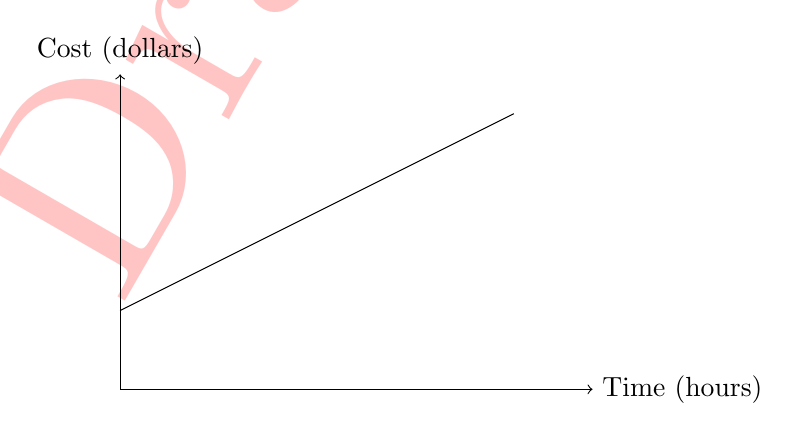
\begin{tikzpicture}
            \draw[->] (0,0) -- (6,0) node[right] {Time (hours)};
            \draw[->] (0,0) -- (0,4) node[above] {Cost (dollars)};
            \draw (0,1) -- (5,3.5);
        \end{tikzpicture}
    \end{center}
    % Page 85
    \item For $2x + 3y = 12$, which equivalent form includes the $y$-intercept as a constant?
    \begin{enumerate}[label=\Alph*)]
        \item $x = -\frac{3}{2}y + 6$
        \item $3y = -2x + 12$
        \item $\frac{2}{3}x - 4 + y = 0$
        \item $y = -\frac{2}{3}x + 4$
    \end{enumerate}
    % Page 86
    \item Line $l$ passes through (-2,3) and (3,13). What is the $y$-coordinate of the $y$-intercept?
    % Page 87
    \item For $5x - 8y = 40$, $y$-intercept is (0,c). What is c?
    % Page 88
    \item What is the $y$-coordinate of the $y$-intercept of $7x = 6 \left( 15 + \frac{9x}{4} - \frac{4y}{7} \right)$?
    % Page 89
    \item Linear function $f$ has negative slope and $y$-intercept (0,k), k > 0. Which must be true?
    \begin{enumerate}[label=\Roman*)]
        \item If $a > b$, then $f(a) < f(b)$
        \item If $a < 0$, then $f(a) > k$
        \item If $a > 0$, then $f(a) > 0$
    \end{enumerate}
    \begin{enumerate}[label=\Alph*)]
        \item I and II
        \item I and III
        \item II and III
        \item I, II, III
    \end{enumerate}
    % Page 90
    \item Daily profit graph: Interpret $y$-intercept.
    \begin{enumerate}[label=\Alph*)]
        \item Price per cake
        \item Cost per cake
        \item Daily running cost
        \item Cost of unsold cakes
    \end{enumerate}
    % Page 91
    \item In $p = 900 - 10t$, interpret 900.
    \begin{enumerate}[label=\Alph*)]
        \item Starting price
        \item Final price
        \item Price increase per second
        \item Auction time
    \end{enumerate}
    % Page 92
    \item In $y = 1.30x - 1.50$, interpret 1.50.
    \begin{enumerate}[label=\Alph*)]
        \item Bank fee in euros
        \item Bank fee in dollars
        \item USD to euro rate
        \item Euro to USD rate
    \end{enumerate}
    % Page 93
    \item The relationship between the daily profit y, in
    dollars, of a bakery and the number of cakes sold
    by the bakery is graphed in the xy-plane below:
    \begin{center}
    \centering
    \includegraphics[width=0.5\linewidth]{Screenshot 2025-06-24 at 19.14.03.png}
    \end{center}
    % Page 94
    \item What does the slope represent?
    \begin{enumerate}[label=\Alph*)]
        \item Price per cake
        \item Profit per cake
        \item Total profit
        \item Cakes for $100 profit$
    \end{enumerate}
    % Page 95
    \item Interpret $y$-intercept.
    \begin{enumerate}[label=\Alph*)]
        \item Price per cake
        \item Cost per cake
        \item Daily running cost
        \item Cost of unsold cakes
    \end{enumerate}
    % Page 96
    \item For $x + 2y = 1$, which form has the $y$-intercept as a constant or coefficient?
    \begin{enumerate}[label=\Alph*)]
        \item $x + 2y - 1 = 0$
        \item $y = \frac{1}{2} - \frac{1}{2}x$
        \item $2y = 1 - x$
        \item $x = 1 - 2y$
    \end{enumerate}
    % Page 97
    \item What is the $y$-intercept of $y = 4x - 1$?
    % Page 98
    \item Which equation matches the graph?
    \begin{center}
        \begin{tikzpicture}
            \draw[->] (-2,0) -- (2,0) node[right] {$x$};
            \draw[->] (0,-1) -- (0,3) node[above] {$y$};
            \draw[domain=-1.5:0.5] plot (\x, {3*\x + 1});
        \end{tikzpicture}
    \end{center}
    \begin{enumerate}[label=\Alph*)]
        \item $y = \frac{1}{3}x + 1$
        \item $y = x + 1$
        \item $y = x + 3$
        \item $y = 3x + 1$
    \end{enumerate}
    % Page 99
    \item Which equation has slope 4 and passes through (0,-3)?
    \begin{enumerate}[label=\Alph*)]
        \item $y = -4x + 3$
        \item $y = -3x + 4$
        \item $y = 4x - 3$
        \item $y = 3x - 4$
    \end{enumerate}
    % Page 100
    \item About $2y - 3x = -4$, which is true?
    \begin{enumerate}[label=\Alph*)]
        \item Negative slope, positive $y$-intercept
        \item Negative slope, negative $y$-intercept
        \item Positive slope, positive $y$-intercept
        \item Positive slope, negative $y$-intercept
    \end{enumerate}
    % Page 101
    \item Line has slope 2 and passes through (0,7). What is $f(2)$?
    \begin{enumerate}[label=\Alph*)]
        \item 9
        \item 11
        \item 14
        \item 16
    \end{enumerate}
    % Page 102
    \item Cereal: 28 oz initially, 2.4 oz eaten/day. Which represents remaining $C$ after $d$ days?
    \begin{enumerate}[label=\Alph*)]
        \item $C = -2.4d + 28$
        \item $C = -2.4d - 28$
        \item $C = 2.4d + 28$
        \item $C = 2.4d - 28$
    \end{enumerate}
    % Page 103
    \item College charges $900/credit + $1000/month room/board. For $x$ credits in 4 months, total charge $y$?
    \begin{enumerate}[label=\Alph*)]
        \item $y = 900x + 4000$
        \item $y = 1000x + 3600$
        \item $y = 3600x + 4000$
        \item $y = \frac{900}{x} + 4000$
    \end{enumerate}
    % Page 104
    \item Linear relationship:
    \begin{center}
        \begin{tabular}{|c|c|}
            \hline
            $s$ & $t$ \\
            \hline
            -5 & 0 \\
            0 & 5 \\
            \hline
        \end{tabular}
    \end{center}
    Which equation?
    \begin{enumerate}[label=\Alph*)]
        \item $t = -s - 5$
        \item $t = -s + 5$
        \item $t = s - 5$
        \item $t = s + 5$
    \end{enumerate}
    % Page 105
    \item Which equation matches the graph?
    \begin{center}
            \centering
            \includegraphics[width=0.5\linewidth]{Screenshot 2025-06-24 at 19.04.45.png}

    \end{center}
    \begin{enumerate}[label=\Alph*)]
        \item $y = -\frac{1}{2}x + 10$
        \item $y = -\frac{1}{2}x + 5$
        \item $y = -2x + 10$
        \item $y = -2x + 5$
    \end{enumerate}
    % Page 106
    \item Equation with slope 2 through (0,-3)?
    \begin{enumerate}[label=\Alph*)]
        \item $y = -3x + 2$
        \item $y = -3x - 2$
        \item $y = 2x + 3$
        \item $y = 2x - 3$
    \end{enumerate}
    % Page 107
    \item $s(p) = 16,000 - 4.5p$ gives free space with $p$ photos (4.5 MB each). If 1500 photos, free space?
    % Page 108
    \item Carol buys 45 figures: first 30 at $d+5$ each, excess at $d$ each. Total cost $A$?
    \begin{enumerate}[label=\Alph*)]
        \item $A = 30d + 45$
        \item $A = 30d + 150$
        \item $A = 45d + 45$
        \item $A = 45d + 150$
    \end{enumerate}
    % Page 109
    \item Line $y = mx + b$ passes through (-20,0) and (0,40). What is $m$?
    % Page 110
    \item $f(x) = px + 8$ has $x$-intercept 4. What is $p$?
    \begin{enumerate}[label=\Alph*)]
        \item -2
        \item 1
        \item $\frac{1}{2}$
        \item 2
    \end{enumerate}
    % Page 111
    \item Equation $2,000 - 61k = 48$ models bird population $k$ years after 1962. Interpret 61.
    \begin{enumerate}[label=\Alph*)]
        \item Population after $k$ years
        \item $k$ when population=48
        \item Difference 1962 and $k$ years
        \item Average decrease per year
    \end{enumerate}
    % Page 112
    \item Linear function $f$:
    \begin{center}
        \begin{tabular}{|c|c|}
            \hline
            $x$ & $f(x)$ \\
            \hline
            8 & 12 \\
            12 & 17 \\
            \hline
        \end{tabular}
    \end{center}
    $f(x) = ax + b$. What is $a + b$?
    % Page 113 (Same as 46)
    \item Values for $h$:
    \begin{center}
        \begin{tabular}{|c|c|}
            \hline
            $x$ & $h(x)$ \\
            \hline
            -7 & -11 \\
            2 & 7 \\
            4 & 11 \\
            \hline
        \end{tabular}
    \end{center}
    What is $h(8)$?
    \begin{enumerate}[label=\Alph*)]
        \item 15
        \item 19
        \item 21
        \item 22
    \end{enumerate}
    % Page 114
    \item Consultant charges $408 first hour + $204/additional hour. Charge for $h$ hours?
    \begin{enumerate}[label=\Alph*)]
        \item $C(h) = 204h + 204$
        \item $C(h) = 204h + 408$
        \item $C(h) = 408h + 204$
        \item $C(h) = 408h + 612$
    \end{enumerate}
    % Page 115
    \item In $17h + 45 = 164$, interpret 164.
    \begin{enumerate}[label=\Alph*)]
        \item One-time fee
        \item Hours worked
        \item Charge per hour
        \item Total charge
    \end{enumerate}
    % Page 116
    \item $p = 873 - 88t$ models pressure after $t$ hours. Pressure after 1 hour?
    \begin{enumerate}[label=\Alph*)]
        \item 829
        \item 785
        \item 741
        \item 697
    \end{enumerate}
    % Page 117 (Same as 7)
    \item Line through (5,7) and (3,11). Which equation?
    \begin{enumerate}[label=\Alph*)]
        \item $f(x) = \frac{1}{2}x + \frac{9}{2}$
        \item $f(x) = -\frac{1}{2}x + \frac{19}{2}$
        \item $f(x) = 2x - 3$
        \item $f(x) = -2x + 17$
    \end{enumerate}
    % Page 118
    \item Graph of $15x + By = 60$. What is $B$?
    \begin{enumerate}[label=\Alph*)]
        \item $\frac{3}{4}$
        \item 3
        \item 4
        \item 20
    \end{enumerate}
    % Page 119
    \item $w(t) = 3.1t - 1.7$ models pig weight at $t$ months. Interpret $w(7) = 20$.
    \begin{enumerate}[label=\Alph*)]
        \item 20 pounds at 7 months
        \item 7 pounds at 20 months
        \item 20 pound increase in month 7
        \item 7 pound increase in month 20
    \end{enumerate}
    % Page 120
    \item Line through (0,2) and (8,0) is $ax + by = 1$. What is $a$?
    % Page 121
    \item Consultant charges $444 first hour + $222/additional hour. Charge for $h$ hours?
    \begin{enumerate}[label=\Alph*)]
        \item $C(h) = 222h + 222$
        \item $C(h) = 222h + 444$
        \item $C(h) = 444h + 222$
        \item $C(h) = 444h + 666$
    \end{enumerate}
    % Page 122
    \item Linear model: 59k in 1991, 222k in 2011, $x$k in 2015. What is $x$?
    % Page 123
    \item Equipment rental: $350 first day + $175/additional day. Cost for $x$ days ($x \leq 5$)?
    \begin{enumerate}[label=\Alph*)]
        \item $y = 175x + 175$
        \item $y = 350x - 175$
        \item $y = 175x + 350$
        \item $y = 350x + 175$
    \end{enumerate}
    % Page 124
    \item $f(t) = 50 + 55t$ models bank account after $t$ deposits. Interpret 55.
    \begin{enumerate}[label=\Alph*)]
        \item Increase of $55 per deposit
        \item Total 55 deposits
        \item Initial $55
        \item $55 after 1 deposit
    \end{enumerate}
    % Page 125
    \item Bus rental: $750 first 2 hours + $50/additional hour. Total cost $1050 for $t$ hours ($t > 2$). Equation?
    \begin{enumerate}[label=\Alph*)]
        \item $750(t - 2) + 50t = 1050$
        \item $750(2t) + 50t = 1050$
        \item $750 + 50(t - 2) = 1050$
        \item $750 + 50(2t) = 1050$
    \end{enumerate}
    % Page 126
    \item Bear weight: 389 lb initially, loses 0.9 lb/day. Days to weigh 380 lb?
    % Page 127 (Same as 12)
    \item Linear profit: $320 at 6 items, $640 at 10 items. Equation?
    \begin{enumerate}[label=\Alph*)]
        \item $f(x) = 180x - 640$
        \item $f(x) = 64x$
        \item $f(x) = 80x - 10$
        \item $f(x) = 80x - 160$
    \end{enumerate}
    % Page 128
    \item Savings: Start $700, deposit $45/week. Amount after 6 weeks?
    \begin{enumerate}[label=\Alph*)]
        \item 430
        \item 745
        \item 751
        \item 970
    \end{enumerate}
    % Page 129
    \item Equipment rental: $64n first day + $32n/additional day. Cost for $x$ days?
    \begin{enumerate}[label=\Alph*)]
        \item $C(x) = 32nx + 32n$
        \item $C(x) = 32nx + 64n$
        \item $C(x) = 64nx + 32n$
        \item $C(x) = 64nx - 32n$
    \end{enumerate}
    % Page 130
    \item Colony: $y = 0.67x + 2.6$ predicts larvae from $x$ worker ants. If $x = 46$, predicted larvae?
    \begin{enumerate}[label=\Alph*)]
        \item 33
        \item 49
        \item 65
        \item 150
    \end{enumerate}
    % Page 131
    \item $P_1 = 10h + 101$, $P_2 = 10d + 311$. Interpret 311.
    \begin{enumerate}[label=\Alph*)]
        \item Total pressure at depth $d$
        \item Pressure increase per meter
        \item Pressure increase for $d$ meters
        \item Total pressure at start of descent
    \end{enumerate}
    % Page 132
    \item Train cars vs passengers:
    \begin{center}
        \begin{tabular}{|c|c|}
            \hline
            Cars & Passengers \\
            \hline
            4 & 164 \\
            6 & 242 \\
            8 & 320 \\
            \hline
        \end{tabular}
    \end{center}
    Which equation?
    \begin{enumerate}[label=\Alph*)]
        \item $39c - p = -8$
        \item $39c - p = 8$
        \item $39p - c = -8$
        \item $39p - c = 8$
    \end{enumerate}
    % Page 133
    \item $17.5x + 28.75y = 530$. How much more per ton of rock than per cubic yard of mulch?
    % Page 134 (Same as 133)
    \item $17.5x + 28.75y = 530$. How much more per ton of rock than per cubic yard of mulch?
    % Page 135
    \item Photosynthetic rate $P(x)$ increases 0.43 when energy increases 5. $P(300) = 9.8$. Equation?
    \begin{enumerate}[label=\Alph*)]
        \item $P(x) = 0.026x + 9.8$
        \item $P(x) = 0.026x + 2$
        \item $P(x) = 9.8x + 0.026$
        \item $P(x) = 9.8x - 2,930.2$
    \end{enumerate}
    % Page 136
    \item Star cluster mass 132.77 quettagrams. Graph models combinations of $x$ M-type and $y$ K-type stars. Estimated mass per star?
    \begin{enumerate}[label=\Alph*)]
        \item 828
        \item 973
        \item 52,992
        \item 79,786
    \end{enumerate}
    % Page 137 (Same as 13)
    \item Adriana's travel time:
    \begin{center}
        \begin{tabular}{|c|c|}
            \hline
            Distance (miles) & Time (minutes) \\
            \hline
            0.06 & 3 \\
            0.28 & 14 \\
            0.34 & 17 \\
            \hline
        \end{tabular}
    \end{center}
    Which equation?
    \begin{enumerate}[label=\Alph*)]
        \item $t = \frac{1}{50}d$
        \item $t = \frac{1}{2}d$
        \item $t = 2d$
        \item $t = 50d$
    \end{enumerate}
    % Page 138
    \item $T(x) = 61 - 8x$ estimates temperature $x$ hours after 10 a.m. Interpret $T(5) = 21$.
    \begin{enumerate}[label=\Alph*)]
        \item 21°F at 5 hours after 10 a.m.
        \item 21°F decrease 5 hours before 10 a.m.
        \item 21°F decrease at 5 hours after 10 a.m.
        \item 21°F at 5 hours before 10 a.m.
    \end{enumerate}
    % Page 139
    \item Linear relationship:
    \begin{center}
        \begin{tabular}{|c|c|}
            \hline
            $x$ & $y$ \\
            \hline
            $-2s$ & 20 \\
            $-s$ & 16 \\
            $s$ & 8 \\
            \hline
        \end{tabular}
    \end{center}
    Which equation?
    \begin{enumerate}[label=\Alph*)]
        \item $sx + 4y = 12s$
        \item $4x + sy = 12s$
        \item $4x + sy = 12$
        \item $sx + 4y = 12$
    \end{enumerate}
    % Page 140
    \item Computer repair: $160 first 2 hours + hourly fee. Total for 4 hours is $240. Cost for $x$ hours ($x \geq 2$)?
    \begin{enumerate}[label=\Alph*)]
        \item $f(x) = 40x + 80$
        \item $f(x) = 40x + 160$
        \item $f(x) = 60x$
        \item $f(x) = 60x + 160$
    \end{enumerate}
    % Page 141
    \item $y$ is 49 more than twice $x$. Equation?
    \begin{enumerate}[label=\Alph*)]
        \item $y = 2x + 49$
        \item $y = 49x + 2$
        \item $y = 51x - 2$
        \item $y = 51x + 49$
    \end{enumerate}
    % Page 142
    \item The graph of line $g$ is shown in the $xy$-plane. Line $k$ is defined by the equation
\[
165x + py = w,
\]
where $p$ and $w$ are constants. If line $k$ is graphed in this $xy$-plane resulting in a system of two linear equations with infinitely many solutions, what is the value of $p + w$?

\begin{center}
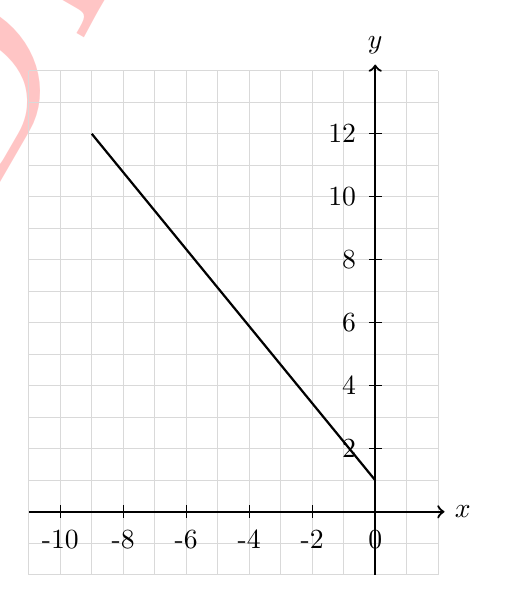
\begin{tikzpicture}[scale=0.4]

    % Draw grid
    \draw[step=1cm, color=gray!30, thin] (-11,-2) grid (2,14);

    % Axes
    \draw[->, thick] (-11,0) -- (2.2,0) node[right] {$x$};
    \draw[->, thick] (0,-2) -- (0,14.2) node[above] {$y$};

    % Axis ticks every 2 units
    \foreach \x in {-10,-8,...,0} {
        \draw (\x,0.2) -- (\x,-0.2);
        \node[below] at (\x,-0.3) {\x};
    }
    \foreach \y in {2,4,...,12} {
        \draw (0.2,\y) -- (-0.2,\y);
        \node[left] at (-0.3,\y) {\y};
    }

    \draw[thick, domain=-9:0] plot (\x, {-11/9*\x + 1});

\end{tikzpicture}
\end{center}
    % Page 143
    \item For $5x - 4y = -20$, which table?
    \begin{enumerate}[label=\Alph*)]
        \item 
            \begin{tabular}{|c|c|c|c|}
                \hline
                $x$ & 0 & 4 & 8 \\
                $y$ & 5 & 10 & 15 \\
                \hline
            \end{tabular}
        \item 
            \begin{tabular}{|c|c|c|c|}
                \hline
                $x$ & 0 & 4 & 8 \\
                $y$ & 15 & 10 & 5 \\
                \hline
            \end{tabular}
        \item 
            \begin{tabular}{|c|c|c|c|}
                \hline
                $x$ & 5 & 10 & 15 \\
                $y$ & 0 & 4 & 8 \\
                \hline
            \end{tabular}
        \item 
            \begin{tabular}{|c|c|c|c|}
                \hline
                $x$ & 5 & 10 & 15 \\
                $y$ & 8 & 4 & 0 \\
                \hline
            \end{tabular}
    \end{enumerate}
    % Page 144
    \item Carpenter: $234 first 3 hours + $65/additional hour. Cost for $x$ hours ($x > 3$)?
    \begin{enumerate}[label=\Alph*)]
        \item $y = 65x + 39$
        \item $y = 234x + 65$
        \item $y = 65x + 234$
        \item $y = 234x + 429$
    \end{enumerate}
    % Page 145
    \item Equipment rental: $230 first day + $115/additional day. Cost for $x$ days ($x \leq 5$)?
    \begin{enumerate}[label=\Alph*)]
        \item $y = 230x + 115$
        \item $y = 230x - 115$
        \item $y = 115x + 230$
        \item $y = 115x + 115$
    \end{enumerate}
    % Page 146
    \item $f(x) = \frac{1}{7}(x - a) + 228$ models car power. At 1896 rpm: 228 bhp; at 4500 rpm: 600 bhp. What is $a$?
    % Page 147
    \item $p(x) = 146 - 5x$ gives paper remaining after $x$ days. Interpret $p(8) = 106$.
    \begin{enumerate}[label=\Alph*)]
        \item Decreased 8 sheets after 106 days
        \item 8 sheets after 106 days
        \item 106 sheets after 8 days
        \item Decreased 106 sheets after 8 days
    \end{enumerate}
    % Page 148
    \item Polar bear ate 25.8 pounds in 6 days. Equation for $y$ pounds in 6 days?
    \begin{enumerate}[label=\Alph*)]
        \item $y = 25.8 + 6$
        \item $y = 25.8$
        \item $y = \frac{25.8}{6}$
        \item $y = 6$
    \end{enumerate}
    % Page 149
    \item $f(x) = 36 - 0.16x$ models water height. Interpret 0.16.
    \begin{enumerate}[label=\Alph*)]
        \item Initial height
        \item Final height
        \item Change in height per day
        \item Days to evaporate
    \end{enumerate}
    % Page 150
    \item System: $y = \frac{2}{7}x + 3$ has infinitely many solutions. If second equation $y = mx + b$, what is $b$?
    \begin{enumerate}[label=\Alph*)]
        \item -3
        \item $-\frac{1}{3}$
        \item $\frac{1}{3}$
        \item 3
    \end{enumerate}
    % Page 151
    \item Large square: 36 cm². Cut out small squares of 4 cm². Area after $x$ cuts?
    \begin{enumerate}[label=\Alph*)]
        \item $f(x) = 36 - 4x$
        \item $f(x) = 36x - 2$
        \item $f(x) = 40x$
        \item $f(x) = 34x$
    \end{enumerate}
    % Page 152
    \item Power washer: $92 first day + $46/additional day. Cost for $d$ days?
    \begin{enumerate}[label=\Alph*)]
        \item $C(d) = 46d + 46$
        \item $C(d) = 46d + 92$
        \item $C(d) = 92d - 46$
        \item $C(d) = 92d + 138$
    \end{enumerate}
    % Page 153
    \item Rover: $y = 390 - 142x$ gives remaining distance $y$ meters after $x$ hours. Interpret 390.
    \begin{enumerate}[label=\Alph*)]
        \item Hours to target
        \item Speed (m/h)
        \item Distance at start
        \item Distance in 1 hour
    \end{enumerate}
    % Page 154
    \item Two students are playing a game. In the
first round, Player 1 answers 33 questions. If
an answer is correct, Player 1 earns 1 point.
If an answer is incorrect, Player 2 will earn
1 point instead. The graph shows y = f(x),
where y is the number of points Player 2 will
earn when x is the number of points Player
1 earns. Which of the following is the best
interpretation of the point (33,0) in this con-
text?
    \begin{enumerate}[label=\Alph*)]
        \item Player 2 earns 33 when Player 1 earns 33
        \item Player 2 earns 0 when Player 1 earns 33
        \item Player 2 earns 33 when Player 1 earns 0
        \item Player 2 earns 0 when Player 1 earns 0
    \end{enumerate}
    % Page 155
    \item Linear relationship:
    \begin{center}
        \begin{tabular}{|c|c|}
            \hline
            $x$ & $y$ \\
            \hline
            -12 & 94 \\
            -6 & 70 \\
            6 & 22 \\
            12 & -2 \\
            \hline
        \end{tabular}
    \end{center}
    Which equation?
    \begin{enumerate}[label=\Alph*)]
        \item $24x + 6y = 46$
        \item $24x + 6y = 276$
        \item $6x + 24y = 46$
        \item $6x + 24y = 276$
    \end{enumerate}
    % Page 156
    \item f(x) = 50x + 8
The given function f estimates the distance
a train has traveled, in kilometers, from a
station in a certain city x hours after crossing the city border. What is the best interpretation of 8 in this context?) models train distance. Interpret 8.
    \begin{enumerate}[label=\Alph*)]
        \item Between the station and the city border, the train traveled an estimated total distance of 8 kilometers  .
        \item Between the station and the city border, the train traveled at an estimated speed of 8 kilometers per hour.
        \item After crossing the city border, the train traveled at an estimated speed of 8 kilometers per hour.
        \item After crossing the city border, the train traveled an estimated total distance of 8 kilometers.
    \end{enumerate}
    % Page 157
    \item The graph of the linear equation $4x + By = 12$ is shown, where $B$ is a constant. What is the value of $B$?
\begin{enumerate}[label=\Alph*)]
    \item $\frac{2}{5}$
    \item 3
    \item 2
    \item 6
\end{enumerate}

\begin{center}
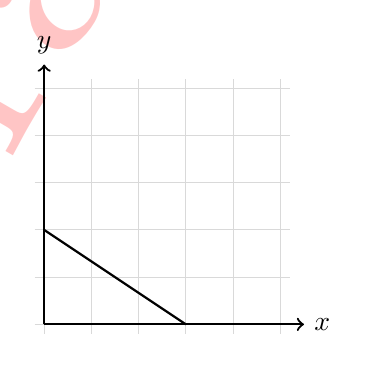
\begin{tikzpicture}[scale=0.6]

    % Grid (no labels)
    \draw[step=1cm, gray!30, thin] (-0.2,-0.2) grid (5.2,5.2);

    % Axes
    \draw[->, thick] (0,0) -- (5.5,0) node[right] {$x$};
    \draw[->, thick] (0,0) -- (0,5.5) node[above] {$y$};

    % Line: goes through (0,2) and (3,0)
    \draw[thick] (0,2) -- (3,0);

\end{tikzpicture}
\end{center}
    % Page 158
    \item Profit $p(x) = 5x - 240$ from selling $x$ stickers. How many to earn $700?
    % Page 159
    \item Bus rental: $850 first 2 hours + $30/additional hour. Total cost $1030 for $t$ hours ($t > 2$). Equation?
    \begin{enumerate}[label=\Alph*)]
        \item $850(t - 2) + 30t = 1030$
        \item $850(2t) + 30t = 1030$
        \item $850 + 30(t - 2) = 1030$
        \item $850 + 30(2t) = 1030$
    \end{enumerate}
    % Page 160
    \item For $7x - 4y = -84$, which table?
    \begin{enumerate}[label=\Alph*)]
        \item 
            \begin{tabular}{|c|c|c|c|}
                \hline
                $x$ & 0 & 4 & 8 \\
                $y$ & 21 & 28 & 35 \\
                \hline
            \end{tabular}
        \item 
            \begin{tabular}{|c|c|c|c|}
                \hline
                $x$ & 0 & 4 & 8 \\
                $y$ & 35 & 28 & 21 \\
                \hline
            \end{tabular}
        \item 
            \begin{tabular}{|c|c|c|c|}
                \hline
                $x$ & 21 & 28 & 35 \\
                $y$ & 0 & 4 & 8 \\
                \hline
            \end{tabular}
        \item 
            \begin{tabular}{|c|c|c|c|}
                \hline
                $x$ & 21 & 28 & 35 \\
                $y$ & 8 & 4 & 0 \\
                \hline
            \end{tabular}
    \end{enumerate}
    % Page 161
    \item A certain open star cluster contains M-type stars and K-type stars. The estimated total mass of M-type and K-type stars in this open star cluster is 129{,}492 quettagrams. The graph shown models the possible combinations of the number of M-type stars, $x$, and K-type stars, $y$, that could be in this open star cluster if all the M-type stars have the same estimated mass and all the K-type stars have the same estimated mass. Based on the graph, which of the following is closest to the estimated mass, in quettagrams, of each M-type star in this cluster?

\begin{enumerate}[label=\Alph*)]
    \item 830
    \item 959
    \item 55{,}622
    \item 73{,}870
\end{enumerate}

\begin{center}
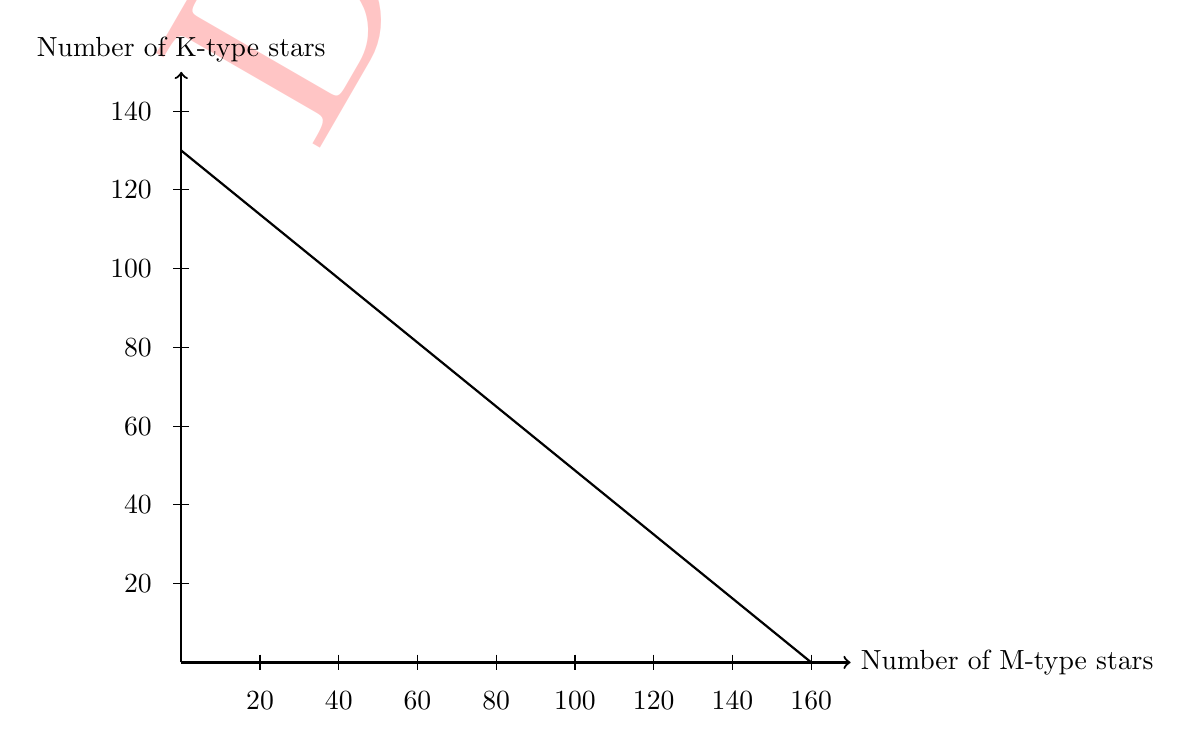
\begin{tikzpicture}[scale=0.05]

    % Axes
    \draw[->, thick] (0,0) -- (170,0) node[right] {Number of M-type stars};
    \draw[->, thick] (0,0) -- (0,150) node[above] {Number of K-type stars};

    % Axis ticks and labels
    \foreach \x in {20,40,...,160} {
        \draw (\x,2) -- (\x,-2);
        \node[below] at (\x,-5) {\x};
    }

    \foreach \y in {20,40,...,140} {
        \draw (2,\y) -- (-2,\y);
        \node[left] at (-5,\y) {\y};
    }

    % Line (approximate): from (0,130) to (160,0)
    \draw[thick] (0,130) -- (160,0);

\end{tikzpicture}
\end{center}
    % Page 162
    \item $f(x) = 39 - 0.18x$ models water height. Interpret 39.
    \begin{enumerate}[label=\Alph*)]
        \item Initial height
        \item Final height
        \item Change per day
        \item Days to evaporate
    \end{enumerate}
    % Page 163
    \item System: $y = \frac{2}{7}x + 3$ has infinitely many solutions. If second equation $y = mx + b$, what is $b$?
    \begin{enumerate}[label=\Alph*)]
        \item -3
        \item $-\frac{1}{3}$
        \item $\frac{1}{3}$
        \item 3
    \end{enumerate}
    % Page 164
    \item Equipment rental: $270 first day + $135/additional day. Cost for $x$ days ($x \leq 5$)?
    \begin{enumerate}[label=\Alph*)]
        \item $y = 135x + 135$
        \item $y = 270x - 135$
        \item $y = 270x + 135$
        \item $y = 135x + 270$
    \end{enumerate}
    % Page 165 (Same as 21)
    \item Roof area vs water drained:
    \begin{center}
        \begin{tabular}{|c|c|}
            \hline
            Area (sq ft) & Water (gallons) \\
            \hline
            2,520 & 4,536 \\
            3,780 & 6,804 \\
            5,040 & 9,072 \\
            \hline
        \end{tabular}
    \end{center}
    Which equation?
    \begin{enumerate}[label=\Alph*)]
        \item $f(x) = 0.6x$
        \item $f(x) = 1.8x$
        \item $f(x) = 2,268.0x$
        \item $f(x) = \frac{x}{6}$
    \end{enumerate}
    % Page 166
    \item Museum: $22/person first 25 + $14/additional. Charge for $n$ people ($n \geq 25$)?
    \begin{enumerate}[label=\Alph*)]
        \item $f(n) = 14n + 200$
        \item $f(n) = 14n + 22$
        \item $f(n) = 14n + 550$
        \item $f(n) = 36n - 350$
    \end{enumerate}
    % Page 167
    \item $y$ is 49 more than twice $x$. Equation?
    \begin{enumerate}[label=\Alph*)]
        \item $y = 2x + 49$
        \item $y = 49x + 2$
        \item $y = 51x - 2$
        \item $y = 51x + 49$
    \end{enumerate}
    % Page 168
    \item The graph of line $g$ is shown in the $xy$-plane. Line $k$ is defined by the equation
\[
165x + py = w,
\]
where $p$ and $w$ are constants. If line $k$ is graphed in this $xy$-plane resulting in a system of two linear equations with infinitely many solutions, what is the value of $p + w$?

\begin{center}
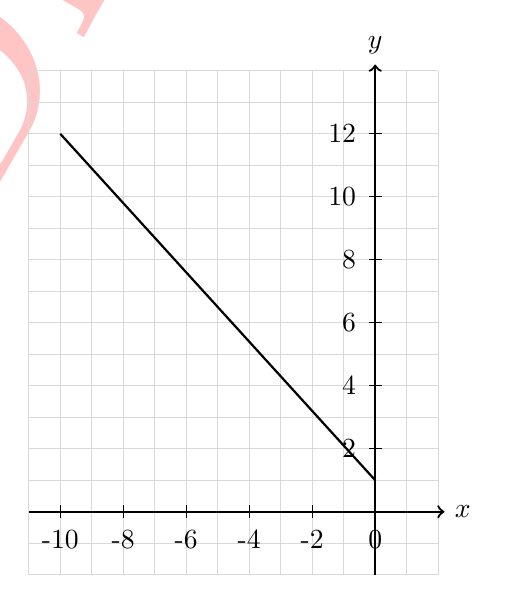
\begin{tikzpicture}[scale=0.4]

    % Draw grid
    \draw[step=1cm, color=gray!30, thin] (-11,-2) grid (2,14);

    % Axes
    \draw[->, thick] (-11,0) -- (2.2,0) node[right] {$x$};
    \draw[->, thick] (0,-2) -- (0,14.2) node[above] {$y$};

    % Axis ticks every 2 units
    \foreach \x in {-10,-8,...,0} {
        \draw (\x,0.2) -- (\x,-0.2);
        \node[below] at (\x,-0.3) {\x};
    }
    \foreach \y in {2,4,...,12} {
        \draw (0.2,\y) -- (-0.2,\y);
        \node[left] at (-0.3,\y) {\y};
    }

    % Line g through (-10,12) and (0,1)
    \draw[thick, domain=-10:0] plot (\x, {-11/10*\x + 1});

\end{tikzpicture}
\end{center}
    % Page 169
    \item A bank account was opened with an initial
deposit. Over the next several months, regu-
lar deposits were made into this account and
there were no withdrawals made during this
time. The graph of the function y = f(x)
estimates the account balance, in dollars, in
this bank account x m o n t h s since t h e initial
deposit. To the nearest whole dollar, what is
the amount of the initial deposit estimated
by the graph?
\begin{center}
\begin{tikzpicture}[scale=1]
    % Axes
    \draw[->, thick] (0,0) -- (5.2,0) node[right] {Months};
    \draw[->, thick] (0,0) -- (0,4.2) node[above] {Balance ($)};

    % Ticks on x-axis (Months)
    \foreach \x/\xtext in {1/1, 2/2, 3/3, 4/4} {
        \draw (\x,0.1) -- (\x,-0.1);
        \node[below] at (\x,-0.1) {\xtext};
    }

    % Ticks on y-axis (Balance)
    \foreach \y/\ytext in {0.5/250, 1/450, 1.5/650, 2/850, 2.5/1050, 3/1250, 3.5/1450, 4/1650} {
        \draw (0.1,\y) -- (-0.1,\y);
        \node[left] at (-0.1,\y) {\ytext};
    }

    % Line from initial deposit
    \draw[thick] (0,1) -- (4,2.5); % scaled: 1 = $450, 2.5 = $1050
\end{tikzpicture}
\end{center}
    % Page 170
    \item $F(m) = 7m$ models force. Interpret $F(4) = 28$.
    \begin{enumerate}[label=\Alph*)]
        \item 28 newtons for 4 kg
        \item 4 newtons for 28 kg
        \item 4 newtons for 7 kg
        \item 28 newtons for 7 kg
    \end{enumerate}
    % Page 171
    \item $13x + 14y = 423$ models shirt sales. Interpret $y$.
    \begin{enumerate}[label=\Alph*)]
        \item Number of long-sleeved shirts
        \item Number of short-sleeved shirts
        \item Price of long-sleeved shirt
        \item Price of short-sleeved shirt
    \end{enumerate}
    % Page 172
    \item $f(x) = -40x + 280$ models airplane height. Height at 4 minutes?
    \begin{enumerate}[label=\Alph*)]
        \item 120
        \item 160
        \item 240
        \item 440
    \end{enumerate}
    % Page 173
    \item Train cars vs passengers:
    \begin{center}
        \begin{tabular}{|c|c|}
            \hline
            Cars & Passengers \\
            \hline
            3 & 99 \\
            5 & 161 \\
            10 & 316 \\
            \hline
        \end{tabular}
    \end{center}
    Which equation?
    \begin{enumerate}[label=\Alph*)]
        \item $31c - p = -6$
        \item $31c - p = 6$
        \item $31p - c = -6$
        \item $31p - c = 6$
    \end{enumerate}
    % Page 174
    \item Linear relationship:
    \begin{center}
        \begin{tabular}{|c|c|}
            \hline
            $x$ & $y$ \\
            \hline
            -2 & 19 \\
            0 & 31 \\
            2 & 43 \\
            \hline
        \end{tabular}
    \end{center}
    If $Ax + By = C$, what is $\frac{A}{B}$?
    % Page 175
    \item Rectangular garden: length $x$, width $y$, fencing total 44 feet. Equation?
    \begin{enumerate}[label=\Alph*)]
        \item $2x + 2y = 44$
        \item $x + y = 44$
        \item $2xy = 44$
        \item $xy = 44$
    \end{enumerate}
    % Page 176
    \item Linear profit: $190 at 4 items, $670 at 10 items. Equation?
    \begin{enumerate}[label=\Alph*)]
        \item $f(x) = 180x - 670$
        \item $f(x) = 67x$
        \item $f(x) = 80x - 10x$
        \item $f(x) = 80x - 130$
    \end{enumerate}
    % Page 177
    \item Linear relationship:
    \begin{center}
        \begin{tabular}{|c|c|}
            \hline
            $x$ & $y$ \\
            \hline
            0 & 22 \\
            1 & 23 \\
            2 & 24 \\
            \hline
        \end{tabular}
    \end{center}
    Which equation?
    \begin{enumerate}[label=\Alph*)]
        \item $y = x + 22$
        \item $y = 24x$
        \item $y = 24x + 2$
        \item $y = 22x$
    \end{enumerate}
    % Page 178
    \item Container: 24 mL initially. Faucet adds 0.03 mL every 3 seconds. Volume $v$ after $t$ seconds (multiple of 3)?
    \begin{enumerate}[label=\Alph*)]
        \item $v = 0.01t + 24$
        \item $v = 0.03t + 24$
        \item $v = 0.09t + 24$
        \item $v = 3t$
    \end{enumerate}
    % Page 179 (Multi-part)
    \item Jenny made $x$ cookies/hour for 2 hours, Cara $y$ cookies/hour for 3 hours. Total cookies?
    \begin{enumerate}[label=\Alph*)]
        \item $6xy$
        \item $3x + 2y$
        \item $2x + 3y$
        \item $5xy$
    \end{enumerate}
    % Page 180
    \item $W = 42 - 7d$ models wills left. Interpret 42.
    \begin{enumerate}[label=\Alph*)]
        \item Finish in 42 days
        \item 42 wills/day
        \item 6 wills/hour
        \item Start with 42 wills
    \end{enumerate}
    % Page 181
    \item Skateboard: 8 ft/s at hilltop, 43 ft/s after 3.5 seconds. Acceleration (ft/s²)?
    \begin{enumerate}[label=\Alph*)]
        \item 8
        \item 10
        \item 12
        \item 14
    \end{enumerate}
    % Page 182
    \item Softball team: $75/member + $50 fee. Max members for $780?
    % Page 183
    \item $2.25x + 0.75y = 35$ for avocados and bananas. Interpret 35.
    \begin{enumerate}[label=\Alph*)]
        \item Avocados/week
        \item Money spent/week
        \item Total fruits/week
        \item Difference avocados-bananas
    \end{enumerate}
    % Page 184
    \item 5 burgers with tax: $30.97 (tax $0.22). Cost of 4 burgers without tax?
    \begin{enumerate}[label=\Alph*)]
        \item 18.00
        \item 20.25
        \item 24.60
        \item 28.00
    \end{enumerate}
    % Page 185
    \item $34c + 52t = 1070$ for trucks and cars. If 16 trucks, how many cars?
    % Page 186
    \item John's meal $y$, Matt's $y+6$. Split evenly. Each pays?
    \begin{enumerate}[label=\Alph*)]
        \item $y$
        \item $y + 6$
        \item $y + 3$
        \item $2y + 6$
    \end{enumerate}
    % Page 187
    \item James 40 shares, Danny 35, John 28. Share value $7. Total value?
    \begin{enumerate}[label=\Alph*)]
        \item 441
        \item 476
        \item 721
        \item 796
    \end{enumerate}
    % Page 188
    \item Cupcake company: 146/day in 2020, 12 less than half of last year. Last year average?
    % Page 189
    \item Jamie: pies 20 min, cookies 30 min/tray. Spends 8 hours, twice as many cookie trays as pies. How many cookie trays?
    \begin{enumerate}[label=\Alph*)]
        \item 6
        \item 8
        \item 10
        \item 12
    \end{enumerate}
    % Page 190
    \item Farmer: horses $1800, cows $1100. Budget $17,000, at least 13 animals. Max horses?
    % Page 191
    \item Two positive integers: product 84, smaller = $\frac{1}{2}$ larger + 1. Smaller?
    \begin{enumerate}[label=\Alph*)]
        \item 5
        \item 6
        \item 7
        \item 12
    \end{enumerate}
    % Page 192
    \item Dynamite: Monday 63 more than Tuesday. Total 873 sticks. Tuesday?
    \begin{enumerate}[label=\Alph*)]
        \item 400
        \item 405
        \item 468
        \item 810
    \end{enumerate}
    % Page 193
    \item Danny: $8.50/hour first 40 hours, 1.5 times after. Earned $505.75 last week. Total hours?
    % Page 194
    \item Train model: scale 1 cm : 5 m. Length 7.6 cm. New scale 1 cm : 10 m. New length?
    \begin{enumerate}[label=\Alph*)]
        \item 10 cm longer
        \item 10 cm shorter
        \item Half as long
        \item Twice as long
    \end{enumerate}
    % Page 195
    \item Woody: 13-19 logs/day, Willy: 7-16 logs/day. Days to chuck 175 logs?
    % Page 196
    \item Birthday party: $18,000. Initially $n$ family members split equally. After 3 refuse, each pays $1000 more. What is $n$?
    % Page 197
    \item Julie worked 3 less than twice Bruce's hours. Julie $J$ based on Bruce $B$?
    \begin{enumerate}[label=\Alph*)]
        \item $J = 2B - 3$
        \item $J = 2 - 3B$
        \item $J = 2B + 3$
        \item $J = 3 - 2B$
        \item $J = -2B - 3$
    \end{enumerate}
    % Page 198
    \item Line $r$ is defined by the equation $4x - 5y = 8$. Line $s$ is parallel to line $r$ in the $xy$-plane. What is the slope of line $s$?
    \begin{enumerate}[label=\Alph*)]
        \item $\dfrac{5}{4}$
        \item $\dfrac{4}{5}$
        \item $-4$
        \item $-5$
    \end{enumerate}
    % Page 199
    \item In the $xy$-plane, line $l$ passes through $(0,0)$ and is parallel to $y = 6x + 3$. If line $l$ also passes through $(3,d)$, what is $d$?
    % Page 200
    \item Line $r$ is defined by $4x - 7y = 3$. Line $s$ is parallel to line $r$. What is the slope of line $s$?
    \begin{enumerate}[label=\Alph*)]
        \item $\dfrac{7}{4}$
        \item $\dfrac{4}{7}$
        \item $-4$
        \item $-7$
    \end{enumerate}
    % Page 201
    \item Line $k$ is defined by $y = 6x + 5$. Line $j$ is parallel to line $k$ and passes through $(0,11)$. Which equation defines line $j$?
    \begin{enumerate}[label=\Alph*)]
        \item $y = 6x + 11$
        \item $y = 11x + 5$
        \item $y = -6x + 11$
        \item $y = -11x + 5$
    \end{enumerate}
    % Page 202
    \item Line $k$ is defined by $y = 4x + 1$. Line $j$ is parallel to line $k$ and passes through $(0,5)$. Which equation defines line $j$?
    \begin{enumerate}[label=\Alph*)]
        \item $y = -5x + 1$
        \item $y = 5x + 1$
        \item $y = -4x + 5$
        \item $y = 4x + 5$
    \end{enumerate}
    % Page 203
    \item Line $s$ passes through $(0,0)$ and is parallel to $y = 25x + 5$. If line $s$ also passes through $(2,d)$, what is $d$?
    \begin{enumerate}[label=\Alph*)]
        \item 5
        \item 25
        \item 50
        \item 55
    \end{enumerate}
    % Page 204
    \item Line $r$ is defined by $4x - 3y = 8$. Line $s$ is parallel to line $r$. What is the slope of line $s$?
    \begin{enumerate}[label=\Alph*)]
        \item $-4$
        \item $-3$
        \item $\dfrac{3}{4}$
        \item $\dfrac{4}{3}$
    \end{enumerate}
    % Page 205
    \item Line $p$ is defined by $y = 6x - 8$. Line $s$ is parallel to line $p$. What is the slope of line $s$?
    % Page 206
    \item Line $k$ is defined by $y = 7x + 2$. Line $j$ is parallel to line $k$ and passes through $(0,3)$. Which equation defines line $j$?
    \begin{enumerate}[label=\Alph*)]
        \item $y = 7x + 3$
        \item $y = -3x + 3$
        \item $y = -7x + 3$
        \item $y = 3x + 3$
    \end{enumerate}
    % Page 207
    \item Line $k$ is defined by $y = 6x + \dfrac{1}{9}$. Line $j$ is perpendicular to line $k$. What is the slope of line $j$?
    \begin{enumerate}[label=\Alph*)]
        \item $-9$
        \item $-\dfrac{1}{6}$
        \item $\dfrac{1}{9}$
        \item $6$
    \end{enumerate}
    % Page 208
    \item Line $k$ is shown in the $xy$-plane. Line $j$ (not shown) is perpendicular to line $k$ and passes through $(-12,-19)$. Which equation defines line $j$?
    \begin{center}
        \includegraphics[width=0.5\linewidth]{Screenshot 2025-06-24 at 16.45.48.png}
    \end{center}
    \begin{enumerate}[label=\Alph*)]
        \item $y = \dfrac{2}{3}x - 11$
        \item $y = \dfrac{2}{3}x - 27$
        \item $y = \dfrac{3}{2}x - 11$
        \item $y = \dfrac{3}{2}x - 27$
    \end{enumerate}
    % Page 209
    \item Line $j$ is perpendicular to line $k$. What is the slope of line $j$?
    \begin{center}
        \includegraphics[width=0.5\linewidth]{Screenshot 2025-06-24 at 16.48.12.png}
    \end{center}
    \begin{enumerate}[label=\Alph*)]
        \item $-\dfrac{6}{5}$
        \item $\dfrac{6}{5}$
        \item $6$
        \item $-5$
    \end{enumerate}
    % Page 210
    \item Lines $p$ and $q$ are perpendicular with $y$-intercept $-4$. Line $p$ crosses the $x$-axis at $x=3$. At which $x$ does line $q$ cross the $x$-axis?
    \begin{enumerate}[label=\Alph*)]
        \item $\dfrac{4}{3}$
        \item $-4$
        \item $-\dfrac{3}{4}$
        \item $-\dfrac{16}{3}$
        \item $\dfrac{16}{3}$
    \end{enumerate}
    % Page 211
    \item Line $k$ passes through $(2,4)$ and is perpendicular to $y = \dfrac{2}{3}x - 6$. Which is the equation for line $k$?
    \begin{enumerate}[label=\Alph*)]
        \item $y = \dfrac{3}{2}x - 6$
        \item $y = -\dfrac{3}{2}x + 7$
        \item $y = \dfrac{2}{3}x + 7$
        \item $y = -\dfrac{2}{3}x + 7$
        \item $y = -\dfrac{3}{2}x - 6$
    \end{enumerate}
    % Page 212
    \item Points $(4,10)$ and $(1,31)$ are on line $q$. Line $p$ is perpendicular to line $q$. Which equation could be for line $p$?
    \begin{enumerate}[label=\Alph*)]
        \item $y = 7x + 28$
        \item $y = \dfrac{1}{7}x - \dfrac{5}{2}$
        \item $y = -7x + 10$
        \item $y = -\dfrac{1}{7}x + 2$
    \end{enumerate}
    % Page 213
    \item Line $d$ is parallel to line $f$ with equation $y = \dfrac{3}{5}x + \dfrac{9}{2}$. Which could be the equation of line $d$?
    \begin{enumerate}[label=\Alph*)]
        \item $3x + 5y = 20$
        \item $10x - 6y = 3$
        \item $9x - 15y = 40$
        \item $-5x + 3y = 18$
    \end{enumerate}
    % Page 214
    \item Which equation could be for parallel line $b$?
    \begin{center}
        \includegraphics[width=0.5\linewidth]{Screenshot 2025-06-24 at 16.50.18.png}
    \end{center}
    \begin{enumerate}[label=\Alph*)]
        \item $y = x - 3$
        \item $y = \dfrac{1}{2}x - 2$
        \item $y = 2x + 4$
        \item $y = -2x - 5$
    \end{enumerate}
    % Page 215
    \item Lines $l$ and $k$ are parallel. Equation for $l$ is $x + 4y = -5$, line $k$ passes through $(2,8)$. What is the $x$-intercept for line $k$?
    % Page 216
    \item Lines $l$ and $k$ are parallel. Line $l$ passes through $(-1,-7)$ and $(1,3)$. If $(a,b)$ is on line $k$, which is another point on line $k$?
    \begin{enumerate}[label=\Alph*)]
        \item $(a-1,b-5)$
        \item $(a-1,b+5)$
        \item $(a+5,b+1)$
        \item $(a+5,b-1)$
    \end{enumerate}
    % Page 217
    \item The graphs of $7x + 11y = 100$ and $ax + by = 10b$ are perpendicular. Which pair represents parallel lines?
    \begin{enumerate}[label=\Alph*)]
        \item $7x - 11y = 10$, $ax + by = 10b$
        \item $7x + 33y = 100$, $2ax - 3by = 50b$
        \item $33x - 7y = 100$, $3ax + by = b$
        \item $11x + 7y = 100$, $ax + by = 10b$
    \end{enumerate}
    % Page 218
    \item What is the slope of a line perpendicular to $6x = 4y + 10$?
    \begin{enumerate}[label=\Alph*)]
        \item $-1$
        \item $\dfrac{2}{3}$
        \item $\dfrac{3}{2}$
        \item $-\dfrac{2}{3}$
    \end{enumerate}
    % Page 219
    \item Line $k$ is defined by $3x + 5y = 24$. Line $a$ is perpendicular to line $k$. What is the slope of line $a$?
    % Page 220
    \item $g(x)$ is perpendicular to $f(x)$. Which could define $g(x)$?
    \begin{center}
        \includegraphics[width=0.5\linewidth]{Screenshot 2025-06-24 at 16.51.36.png}
    \end{center}
    \begin{enumerate}[label=\Alph*)]
        \item $g(x) = -2x - 2$
        \item $g(x) = -\dfrac{1}{2}x + 4$
        \item $g(x) = \dfrac{1}{2}x + 2$
        \item $g(x) = 2x - 3$
    \end{enumerate}
    % Page 221
    \item Line $m$ is defined by $y = -\dfrac{3}{5}x + 7$. Line $k$ is perpendicular to $m$ and passes through $(6,13)$. Which equation defines $k$?
    \begin{enumerate}[label=\Alph*)]
        \item $y = \dfrac{5}{3}x + \dfrac{1}{7}$
        \item $y = \dfrac{5}{3}x + 3$
\end{document} 